\section{Feature Comparison}
\label{sec:featurecompare}

The GeoMesa and GeoWave projects contain many features that overlap, and many that do not.
The Venn diagram shown in Figure \ref{venn} is not a complete list of features,
but indicates the significant overlap of the core features of GeoWave and GeoMesa and some of the distinguishing features that set them apart.

\begin{figure}[h!tb]
  \centering
  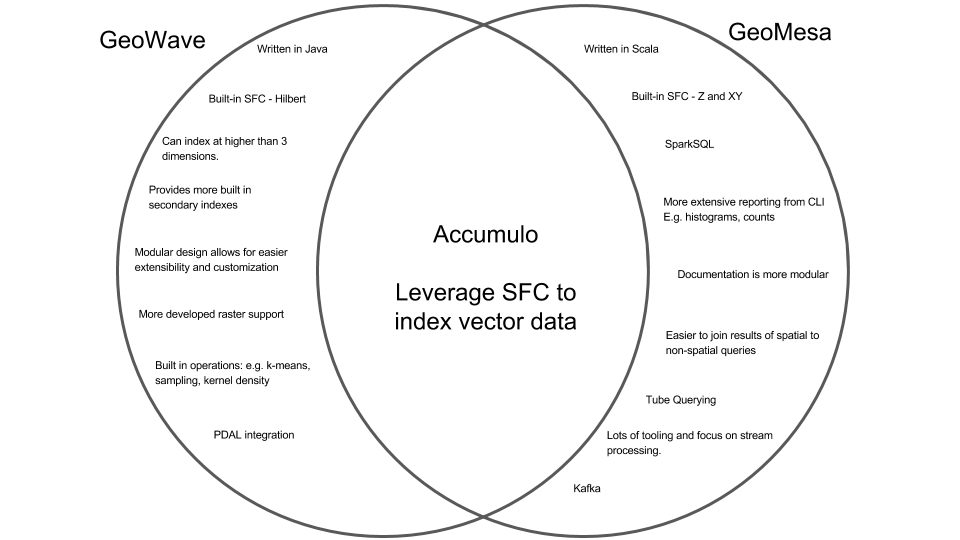
\includegraphics[width=0.60\textwidth]{../docs/img/venn-diagram.png}
  \caption{Venn Diagram of features.}
  \label{venn}
\end{figure}

As is illustrated in the diagram, there is a major overlap when it comes to a core feature of the two projects, namely using space filling curves to index geospatial data in Accumulo.
However, there are many features that differentiate the projects from one another.
Below is a summary table of feature similarities and differences.
A more detailed list of features can be found in Appendix \ref{appendix:features}: Details of GeoMesa and GeoWave features.

{\small
  \begin{longtable}{ | l | c c | }
    \hline & GeoMesa & GeoWave \\ \hline \endfirsthead
    \hline & GeoMesa & GeoWave \\ \hline \endhead
    \hline \multicolumn{3}{|r|}{{Continued on next page}} \\ \hline \endfoot

    \endlastfoot

    \multicolumn{3}{| l |}{INGEST/INPUT} \\ \hline
    Datastore for Accumulo & \checkmark & \checkmark \\
    Ingest vectors & \checkmark & \checkmark \\
    Predefined \texttt{SimpleFeatureTypes} & \checkmark & \checkmark \\
    GDELT & \checkmark & \checkmark \\
    GeoLife & \checkmark & \checkmark \\
    geonames & \checkmark & \\
    gtd & \checkmark & \\
    nyctaxi & \checkmark & \\
    osm-gpx & \checkmark & \\
    tdrive & \checkmark & \checkmark \\
    twitter & \checkmark & \\
    avro & & \checkmark \\
    geotools-vector & & \checkmark \\
    gpx & & \checkmark \\
    stanag4676 & & \checkmark \\
    Ingest rasters & \checkmark & \checkmark \\
    tif & \checkmark & \\
    geotiff & \checkmark & \\
    dt0 & \checkmark & \\
    dt0 & \checkmark & \\
    dt2 & \checkmark & \\
    geotools-raster & & \checkmark \\
    GEOMESA convert tools & \checkmark & \\
    delimited text & \checkmark & \\
    avro & \checkmark & \\
    json & \checkmark & \\
    xml & \checkmark & \\
    GeoMesa Stream & \checkmark & \\
    storm/kafka ingest & \checkmark & \checkmark \\

    \hline \multicolumn{3}{| l |}{BACKENDS} \\ \hline
    Accumulo & \checkmark & \checkmark \\
    HBase & \checkmark & \checkmark \\
    Integration
    mrgeo (reading) & & \checkmark \\
    GeoTrellis & & \checkmark \\
    via c++ bindings - pdal mapnik & & \checkmark \\
    Data Processing
    generate rdd of simple features & \checkmark & \\
    spark sql & \checkmark & \\
    geo-mesa jobs - custom M/R jobs & \checkmark & \\
    Query against Accumulo store & \checkmark & \\
    heatmap from cql & \checkmark & \\
    compute state from cql results & \checkmark & \\
    tube selection & \checkmark & \\
    proximity search & \checkmark & \\
    query $k$-nearest neighbors given point & \checkmark & \checkmark \\
    identify unique valus from cql query & \checkmark & \\
    convert points to lines & \checkmark & \\
    $k$-means & & \checkmark \\
    jump method ($k$ discovery) & & \checkmark \\
    sampling & & \checkmark \\
    kernel density estimation & & \checkmark \\
    clustering & & \checkmark \\
    convex hulls of cluster & & \checkmark \\
    dbscan & & \checkmark \\
    spark support & & \checkmark \\

    \hline \multicolumn{3}{| l |}{PRIMARY INDICES} \\ \hline
    default & \checkmark & \\
    xz3 & \checkmark & \\
    xz2 & \checkmark & \\
    z3 & \checkmark & \\
    z2 & \checkmark & \\
    record & \checkmark & \\
    Hilbert & & \checkmark \\

    \hline \multicolumn{3}{| l |}{SECONDARY INDICES} \\ \hline
    attribute & \checkmark & \\
    ST & \checkmark & \\
    Cost-Based Optimization (selects index) & \checkmark & \\
    Numerical & & \checkmark \\
    Temporal & & \checkmark \\
    Textual & & \checkmark \\
    User-Defined & & \checkmark \\
    No Cost-based Optimization & & \checkmark \\

    \hline \multicolumn{3}{| l |}{OUTPUT} \\ \hline
    Accumulo & \checkmark & \\
    reader for querying datastore in java & \checkmark & \\
    produce collection of features from datastore & \checkmark & \\
    direct map/reduce exports & \checkmark & \\
    command line tools & \checkmark & \\
    serialize export vectors & \checkmark & \\
    csv & \checkmark & \\
    shapefile & \checkmark & \\
    geojson & \checkmark & \\
    gml & \checkmark & \\
    bin & \checkmark & \\
    avro & \checkmark & \\
    GeoServer Plugin & & \checkmark \\
    Query - RDD & & \checkmark \\
    Query - Iterator & & \checkmark \\

    \hline \multicolumn{3}{| l |}{OTHER FEATURES} \\ \hline
    gpm native api & \checkmark & \\
    hbase backend & \checkmark & \\

    \hline
    \caption{Feature Summary}
    \label{table:summary}
  \end{longtable}
}


\subsection{Generality of the Architecture}
\label{sec:featurecompare:generality}

A major difference between the projects is the generality of the architectures when it comes to supporting
various backends\footnote{Backend refers to the specific mechanism for storing vector, data and the related geospatial index (ex: Accumulo, HBase).}
and indexing strategies.
GeoWave API has a focus on being an N-Dimensional indexing mechanism for arbitrary backends.
The fact that this document focuses on its ability to handle geospatial data ($2$-Dimensional spatial and $3$-Dimensional spatiotemporal data) is only based on the currently known GeoWave use cases.
However, the project aims at supporting data with arbitrary dimensionality.
GeoMesa API, on other hand, is directly tailored to geospatial indexing allowing for clearer interface, implementation, and paths for optimization.

GeoWave specifically is designed around abstractions that remain agnostic about the storage and access implementations.
This could provide more flexibility for developing backend support, which might explain why GeoWave HBase support is more mature than GeoMesa's.
GeoMesa focuses on using GeoTools' abstractions, and thus is more dependent on GeoTools as a base library.
GeoMesa also focuses less on dealing with abstractions; this may have an effect that features written for one backend are difficult to translate to another backend.
However, dealing with less abstraction can be more straightforward, and some developers may find it easier to understand and work with the GeoMesa API.

\section{Language}
\label{sec:featurecompare:language}

GeoMesa is developed using Scala, and GeoWave is developed using Java.
Both Scala and Java are languages in which the source compiles down to Java Virtual Machine (JVM) bytecode, which is executed on top of the same JVM.
This means that both projects can use the same dependencies, as can be observed by each project's reliance on GeoTools (a Java based geospatial library) for some of its features, including a core data type: the GeoTools \texttt{SimpleFeature}.
However, the differences between the Scala and Java languages are many, and it remains one of the biggest differences between the projects.

%% And user familiarity with the implementation languages should be considered as factor.
%% We will address this from the perspective of Java developers as they are a larger group of potential users.
%% GeoWave uses standard and well structured Java composition and design patterns both in its API and implementation and should provide few surprises for Java developers.
%% GeoMesa, though written in Scala, implements a GeoTools API that allows Java developers to easily use GeoMesa functionality without having to write Scala.
%% Java interoperability is a core design concern in GeoMesa API as evidenced by tutorial code being provided exclusively in Java.
%% This has limits, however, as developers investigating stack traces and exploring the GeoMesa implementation will encounter Scala.
%% Being Scala developers we can comment that GeoMesa codebase uses direct dialect of Scala, eschewing advanced language features and staying close to Java patterns which optimizes its readability for such a developer.
%% Ultimately the feasibility of this should be part of individual team evaluation when adopting either project.

\subsection{Accumulo Indexing}
\label{sec:featurecompare:indexing}

The two projects approach indexing in Accumulo in a similar way, but there are some key differences.

\subsubsection{Choice of Space Filling Curve}
\label{sec:featurecompare:indexing:curve}

GeoMesa supports the space filling curve indices named Z-order and XZ indices, while GeoWave supports Hilbert curves.
These space filling curve implementations have different properties that affect performance, such as the number of false positives returned and number of duplicate entries to be indexed.
You can read more about the differences in performance characteristics in Appendix \ref{appendix:planning}: Details of Performance Test Conclusions.

\subsubsection{Sharding}
\label{sec:featurecompare:indexing:sharding}

By default, GeoMesa uses ``sharding'', a technique of prefixing indices with a discrete number of shard IDs in order to better distribute the data across nodes of a cluster.
There is a trade-off between increasing distribution while decreasing locality.
Index sharding leads to more even per-query cluster resource utilization, which covers the common use cases GeoWave has the ability to shard, although in GeoWave it's called partitioning the data.
You can create a compound index with any of the GeoWave indexing strategies in order to partition.
Unlike GeoMesa, GeoWave partitioning is not enabled by default.
It is also configurable: you can decide on the number of partitions (i.e. shards) you want, and determine whether or not it's a round robin or hashing strategy that determines the partition ID.
GeoMesa's sharding seems to only use a hashing algorithm and a non-configurable number of shards.
In our benchmarks we had to enable index partitioning in GeoWave in order to improve its performance and make the benchmarks comparable.

\subsubsection{Periodicity}
\label{sec:featurecompare:indexing:periodicity}

To get around the problem of unbounded dimensions, such as time, the concept of ``periodicity'' is used in both GeoMesa and GeoWave.
This feature is similar to a shard, in that it prefixes an index with some ID.
A simple way to think of periodicity is that it bins each space filling curve into one period; for example, for one week.
In GeoWave, you can configure any dimension to have a periodicity of a configurable length.
With GeoMesa, you can configure the periodicity of the time dimension to day, week, month, or year.

\subsubsection{Tiered indexing vs XZ index}
\label{sec:featurecompare:indexing:versus}

GeoMesa uses an XZ index to handle non-point data, which allows the data to be stored at specific space filling curve resolutions based on the the size of the geometry.
GeoWave uses a technique called tiered indexing to handle this issue.
The technical differences between the two approaches are beyond the scope of this document.
Broadly, they have comparable theoretical performance with tiering being more flexible of the two, allowing for more use-case specific optimization.
However one major difference between the two approaches is that the XZ approach does not store any duplicates of data, while the tiered strategy can store up to four copies of an entry.

\subsection{Other features}
\label{sec:featurecompare:other}

This section gives a summary of features that are either found in one project and not the other,
or are found in both projects with considerable differences.


\subsubsection{Features Found in GeoWave and not in GeoMesa}
\label{sec:featurecompare:other:wave}

\begin{itemize}
\item Integration with Mapnik
\item Integration with PDAL for reading and writing point cloud data from/to GeoWave
\item Time interval queries: The ability to index data that exists within an interval of time, and query for intersecting intervals
\item Pixel-level subsampling: A visualization performance optimization that returns a subset of the resulting data based on pixel width
\item DBScan clustering
\end{itemize}


\subsubsection{Features Found in GeoMesa and not in GeoWave}
\label{sec:featurecompare:other:mesa}

\begin{itemize}
\item Tube selection analysis: Given a collection of points (with associated times), return a similar collections of points in terms of where the lines connecting said points exist
\item Loose bounding box queries: Return all points where the index matches the space filling curve index query, and skip secondary filtering
\item JSON configurable ingest tooling
\item Cassandra backend (alpha support)
\item Google BigTable support (marked experimental)
\item Kafka GeoTools DataStore
\item Cost-based query optimization
\item Querying for a subset of SimpleFeature attributes and only returning the necessary data
\end{itemize}


\subsubsection{Raster Support}
\label{sec:featurecompare:other:raster}

Both projects have some level of raster support; however, GeoWave's raster support appears to be more mature than GeoMesa's.
According to GeoMesa's documentation, rasters must be pre-tiled to a specific size, projection, have non-overlapping extents, and must only single band rasters.
GeoWave supports multiband rasters, and includes tiling and merging strategies that allow you to ingest rasters that are not pre-tiled.
While GeoWave's raster support is more mature than GeoMesa's, both project's support of raster data is not entirely mature; for instance,
there is no support for anything but spatial rasters (i.e. you cannot ingest spatiotemporal raster data such as timestamped imagery).

  
\subsubsection{HBase Backend}
\label{sec:featurecompare:other:hbase}

Both projects have support for an HBase backend; however, GeoWave's support for HBase is more mature.
The GeoWave development team has expressed the amount of work that has gone into trying to match the performance of the HBase backend to that of their Accumulo backend.
The GeoMesa team expressed that there has not yet been an equal level of effort to achieve relative parity between their Accumulo and HBase backends.


\subsubsection{Attribute/Secondary indexing}
\label{sec:featurecompare:other:secondary}

GeoMesa and GeoWave both have features around secondary indexing that are quire different.
A detailed comparison of those features for both GeoMesa and GeoWave can be found in Appendix A: Details of GeoMesa and GeoWave features.

